\documentclass[]{article}
\usepackage[spanish]{babel}
\usepackage{graphicx}
\usepackage{float} 
\usepackage{standalone}
\usepackage{adjustbox}
\usepackage{longtable} 
\usepackage{booktabs} 
\usepackage{rotating} 
\usepackage{float}
\usepackage{fontawesome} % Paquete para íconos
\usepackage{amsmath}
\usepackage{enumitem}
\setlength{\parindent}{0pt} 
\graphicspath{{C:/Users/USER/Documents/econometria/tarea1/plot/}}
\usepackage[letterpaper]{geometry}


%opening
\title{Problem Set 1}
\author{Tannya Mainato \and Alan Del Rosario \and Mariuxi Gualán}
\date{2024}

\begin{document}
\maketitle
\section*{Pregunta 1}

Gráfica de cada línea:

\begin{enumerate}[label=\alph*)]
	\item $\sqrt{3+2x}$ 
	\begin{figure}[H]
		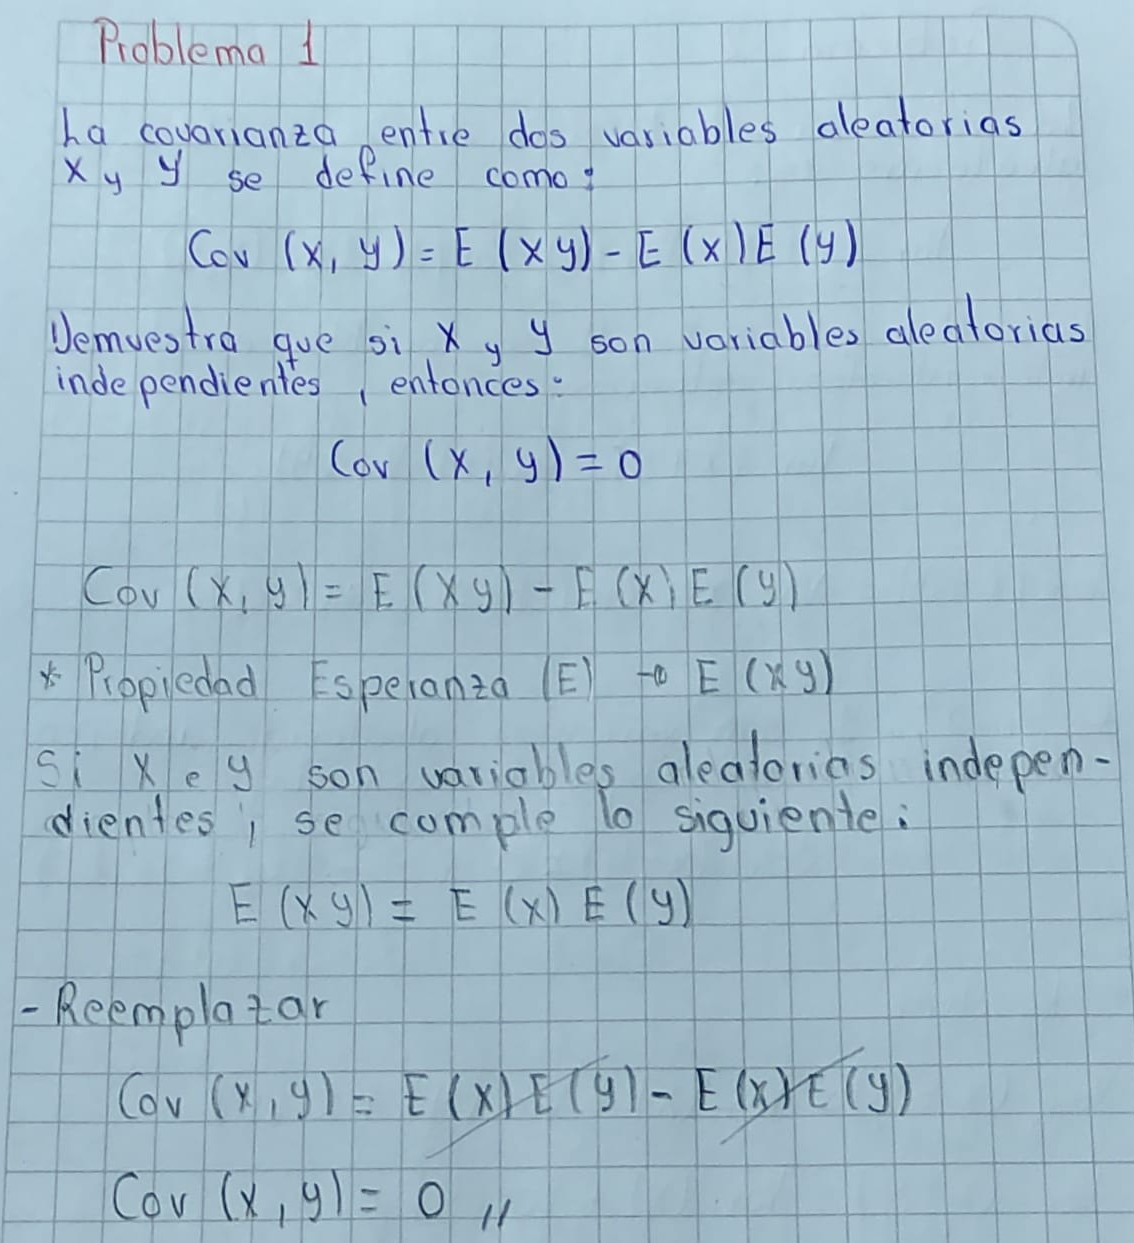
\includegraphics[width=0.84\linewidth]{/Pregunta_1/1_a.jpg}
	\end{figure}
	\item $y=-2-\frac{1}{2}x$
	\begin{figure}[H]
		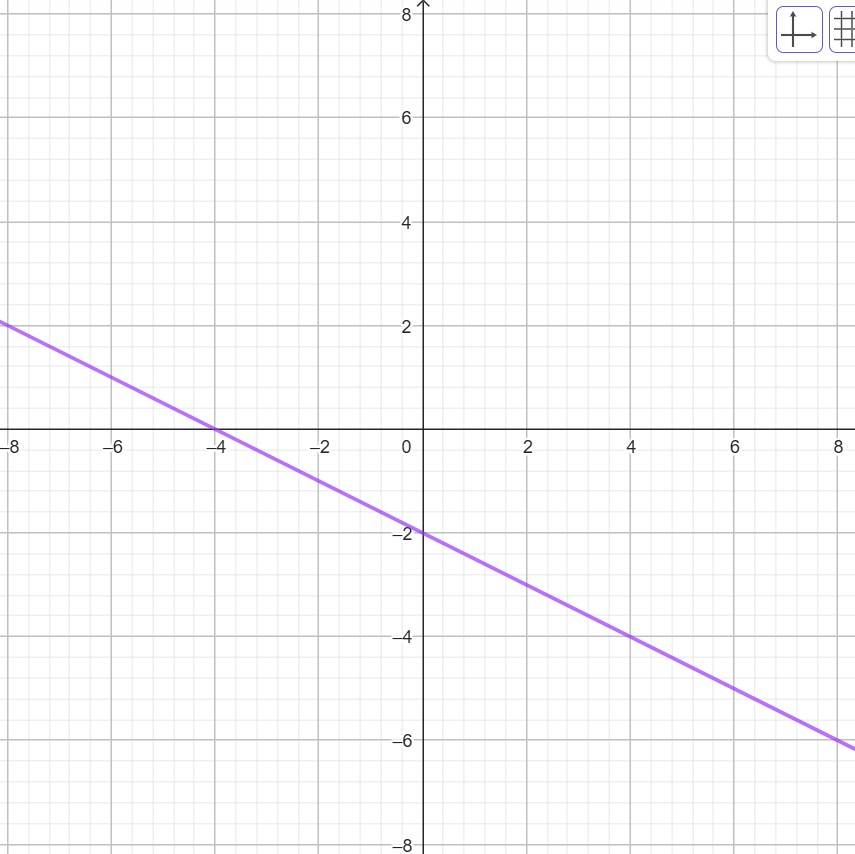
\includegraphics[width=0.84\linewidth]{/Pregunta_1/1_b.jpg}
	\end{figure}
\end{enumerate}

\section*{Pregunta 2}
Encuentra la ecuación de la línea recta que pasa por los puntos:

\begin{enumerate} [label=\alph*)]
	\item $(0,3)$ y $(4,0)$\\
	y=mx+b $\rightarrow$ y=-3/4x+3
	\\
	\textbf{Valor de la pendiente}
	\\\\
	$m = \frac{Y_2 - Y_1}{X_2 - X_1}$
	\\\\
	$m = \frac{0-3}{4-0}$
	\\\\
	m=-$\frac{3}{4}$
	\\
	\textbf{Valor de intercepto}
	\\
	\textbf{B} toma el valor de $y$ cuando $x$ es cero.
	\\
	Punto: (0,3)\\
	b=3\\
	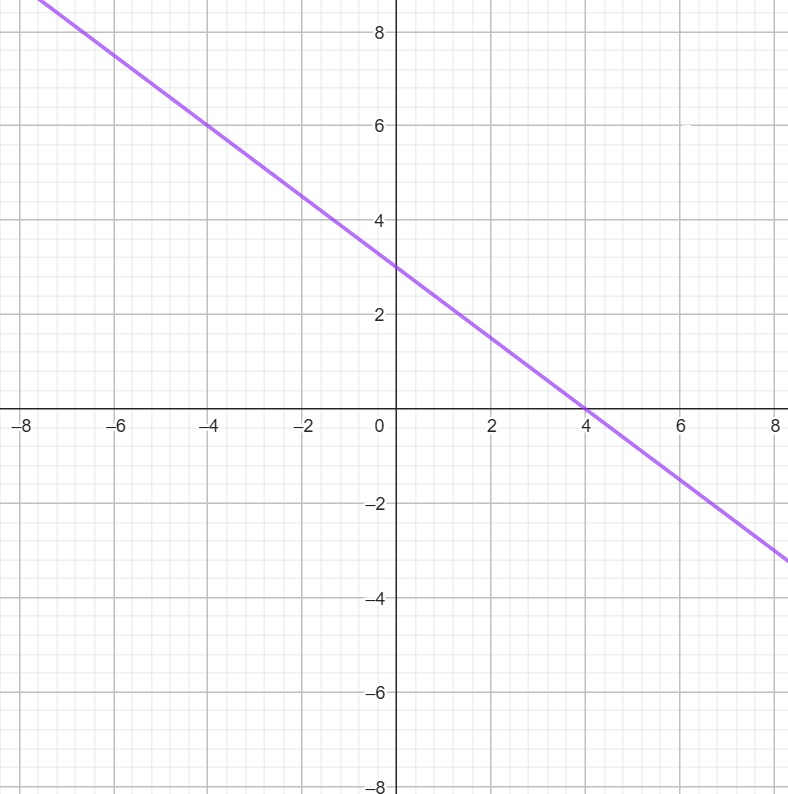
\includegraphics[width=0.6\linewidth]{/Pregunta_2/2_a.jpg}
	\item $(2,-3)$ y $(6,5)$
	\\
	y=mx+b $\rightarrow$ y=2x-7
	\\
	\textbf{Valor de la pendiente}
	\\\\
	$m = \frac{Y_2-Y_1}{X_2-X_1}$
	\\\\
	$m = \frac{5-(-3)}{6-2}$
	\\\\
	m = 2\\
	\textbf{Valor del intercepto}\\
	Punto: (6,5) en la función $y = mx+b$\\\\
	5=2(6)+b\\\\
	b=-7\\
	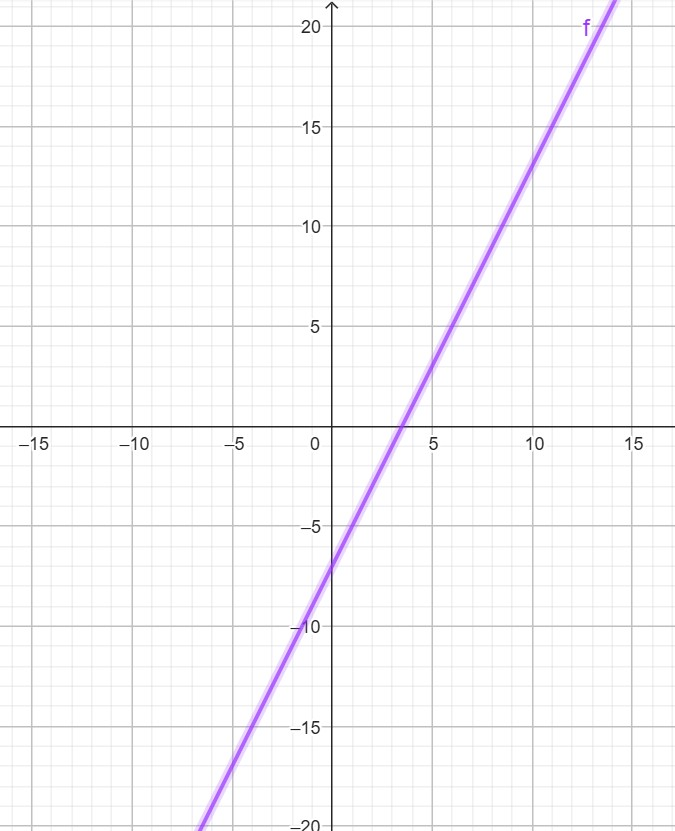
\includegraphics[width=0.6\linewidth]{/Pregunta_2/2_b.jpg}
\end{enumerate}
 
\section*{Pregunta 3}
Dada la ecuación: 

$$y=-1+2x_1-\frac{1}{2}x_2+3x_3$$

Encuentra el valor de $y$ cuando $x_1=3$, $x_2=4$ y $x_3=5$.

Sustituyendo los valores dados:\\\\
$y = -1+2(3)-\frac{1}{2}(4)+3(5)$\\\\
$y = -1+6-2+15$\\\\
$y=\textbf{18}$

\section*{Pregunta 4}
Calcula las siguientes sumatorias:

\begin{enumerate}[label=(\alph*)]
	\item $\sum_{i=1}^{5}i$\\\\
	La sumatoria de $i$ desde 1 hasta 5 es:\\\\
	$\sum_{i=1}^{5}=1+2+3+4+5$\\\\
	$\sum_{i=1}^{5}=\textbf{15}$\\\\
	\item $\sum_{i=1}^{6}2i$\\\\
	Se multiplica para el 2, valores del 1 al 6:\\\\
	$\sum_{i=1}^{6}2i=2(1) + 2(2) + 2(3) + 2(4) + 2(5) + 2(6)=2(1 + 2 + 3 + 4 + 5 + 6)$\\\\
	$\sum_{i=1}^{6}2i=2 + 4 + 6 + 8 + 10 + 12$\\\\
	$\sum_{i=1}^{6}2i=\textbf{42}$\\\\
	\item $\sum_{i=1}^{4}(3i-1)$\\\\
	$\sum_{i=1}^{4}(3i-1)=(3(1)-1)+(3(3)1)+(3(4)-1)$\\\\
	$\sum_{i=1}^{4}(3i-1)=(3-1)+(6-1)+(9-1)+(12-1)$\\\\
	$\sum_{i=1}^{4}(3i-1)=2+5+8+11$\\\\
	$\sum_{i=1}^{4}(3i-1)=\textbf{26}$\\\\
	\item $\sum_{i=1}^{3}(2i+1)^2$\\\\
	$\sum_{i=1}^{3}(2i+1)^2$\\\\
	$\sum_{i=1}^{3}(2i+1)^2=(2(1)+1)^2 + (2(2)+1)^2 + (2(3)+1)^2$\\\\
	$\sum_{i=1}^{3}(2i+1)^2=(2 + 1)^2 + (4 + 1)^2 + (6 + 1)^2$\\\\
	$\sum_{i=1}^{3}(2i+1)^2=(3)^2+(5)2+(7)^2$\\\\
	$\sum_{i=1}^{3}(2i+1)^2=9+25+49$\\\\
	$\sum_{i=1}^{3}(2i+1)^2=\textbf{83}$
\end{enumerate}

\section*{Pregunta 5}
¿Cuál es la sumatoria de $\sum_{i=1}^{5}1$?

\begin{figure}[H]
	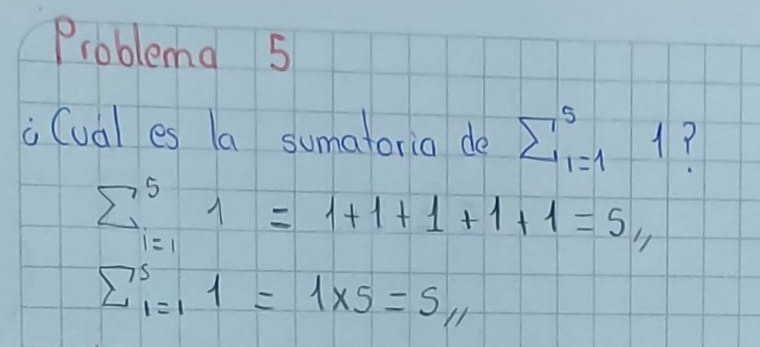
\includegraphics[width=0.7\linewidth]{/Pregunta_5/5_a.jpg}
\end{figure}

\section*{Pregunta 6}
Calcula las siguientes derivadas. No es necesario simplificar.

\begin{enumerate}[label=(\alph*)]
	\item Encuentra $\frac{dy}{dx}$ de $y=3x^2$
	\item Encuentra $\frac{dy}{dx}$ de $y=4x^{-3}+2$
	\begin{figure}[H]
		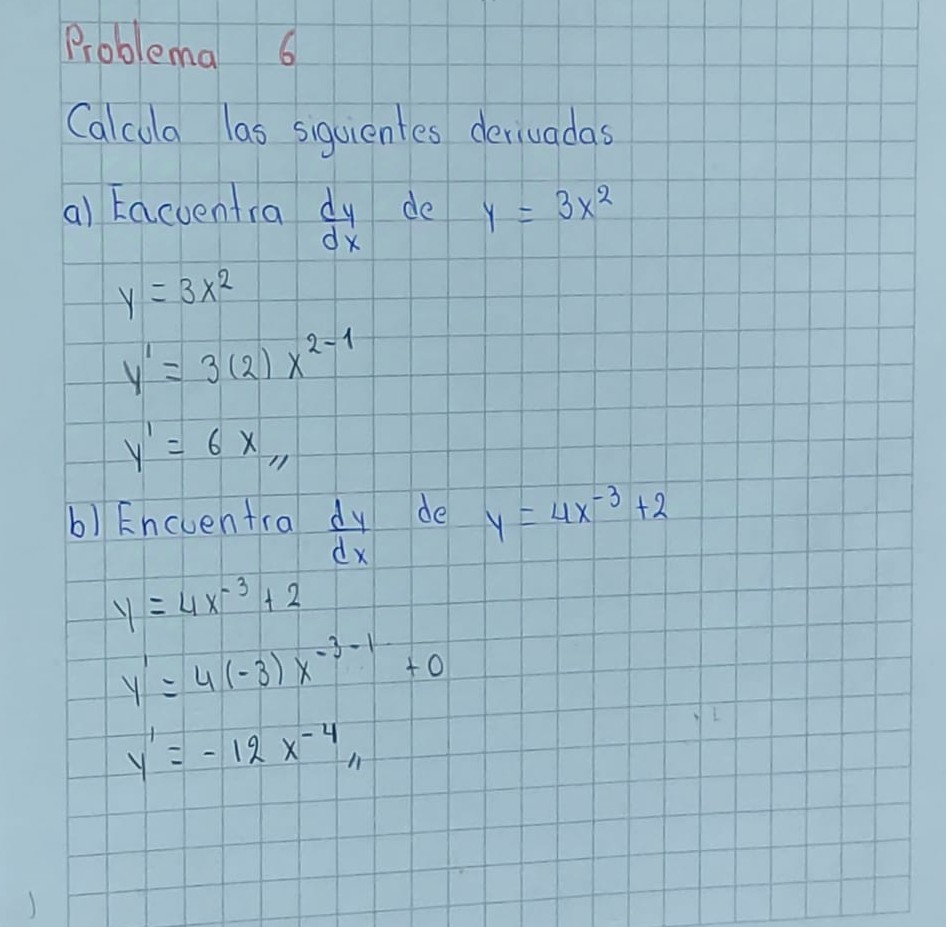
\includegraphics[width=0.72\linewidth]{/Pregunta_6/6_a_b.jpg}
	\end{figure}
	\item Encuentra $\frac{df(x)}{dx}$ de $f(x)=2x^{-1/2} - 6x$
	\item Encuentra $\frac{df(x)}{dx}$ de $f(x)=3x^2-4x+1$
	\begin{figure}[H]
	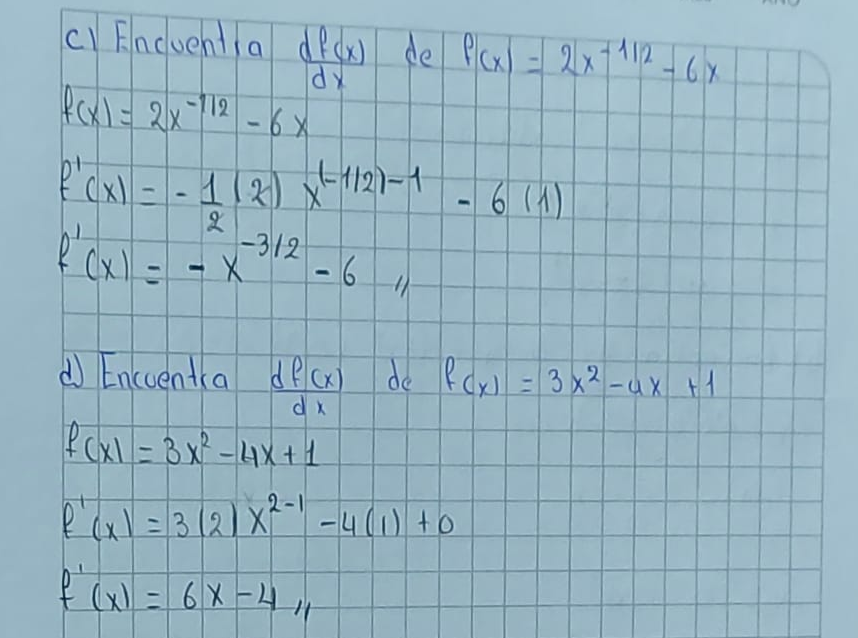
\includegraphics[width=1\linewidth]{/Pregunta_6/6_c_d.png}
	\end{figure}
\end{enumerate}

\section*{Pregunta 7}
Calcula las siguientes derivadas utilizando la regla de la cadena. No es necesario simplificar.

\begin{enumerate}[label=\alph*]
	\item Encuentra $\frac{dy}{dx}$ de $y=(2x+3)^5$
	\begin{figure}[H]
		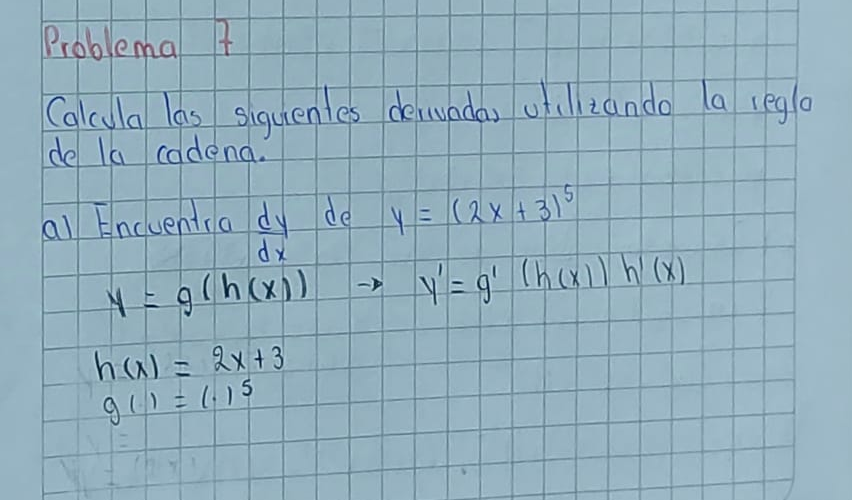
\includegraphics[width=1\linewidth]{/Pregunta_7/7_a.png}
	\end{figure}
	\item Encuentra $\frac{dy}{dy}$ de $y=(3x^2+2x)^3$
	\item Encuentra $\frac{df(x)}{dx}$ de $f(x)=(2x^3-3x^2+1)^2$
	\begin{figure}[H]
	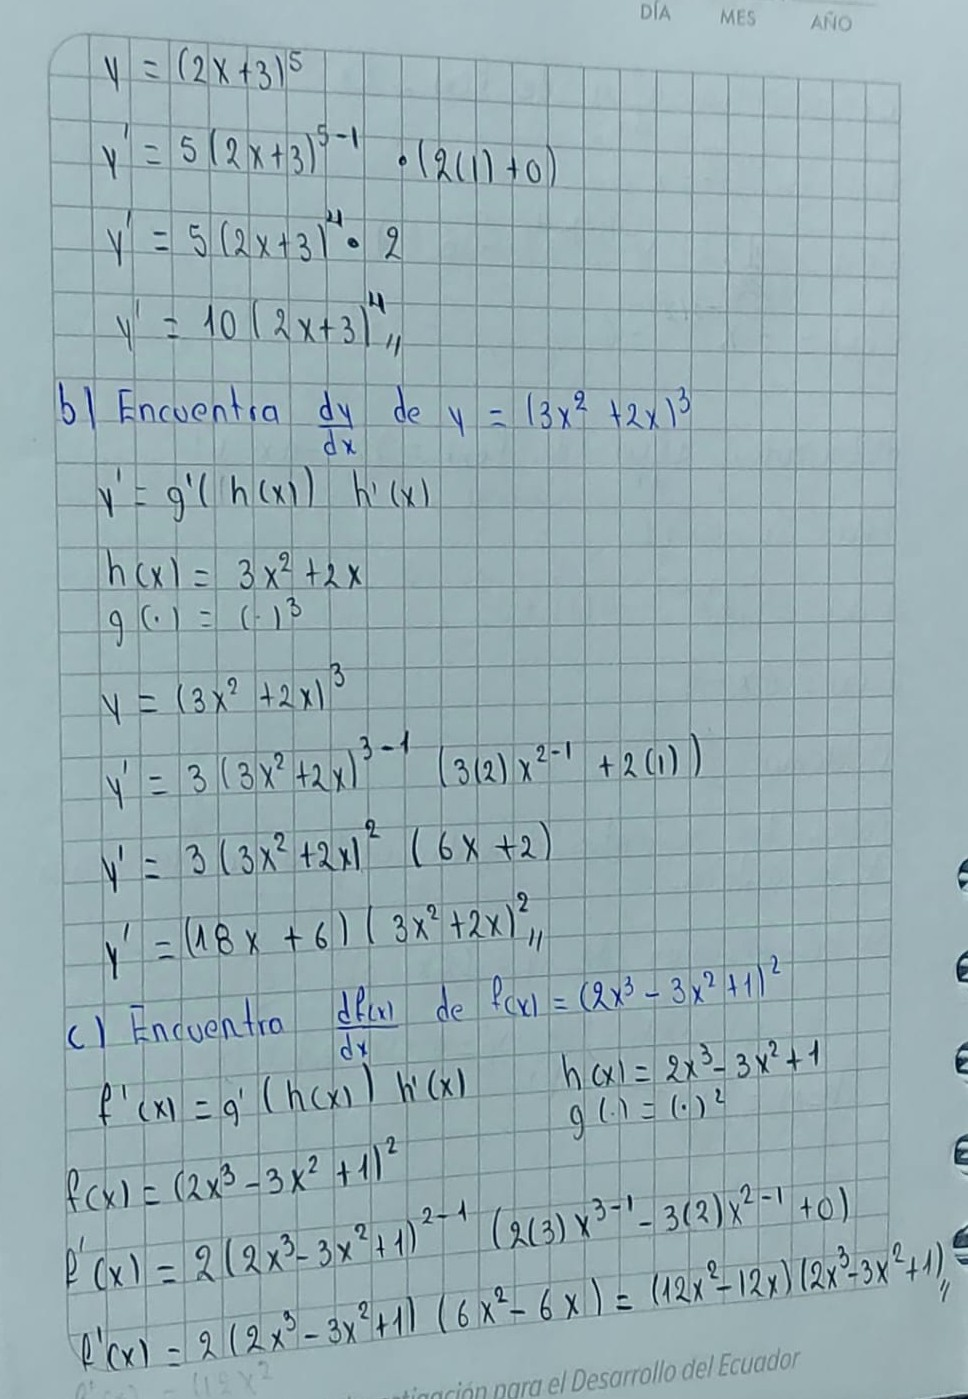
\includegraphics[width=1\linewidth]{/Pregunta_7/7_b_c.png}
	\end{figure}
	\item Encuentra $\frac{df(x)}{dx}$ de $f(x)=(2x^2+5)^{\frac{1}{2}}$ 
	\begin{figure}[H]
		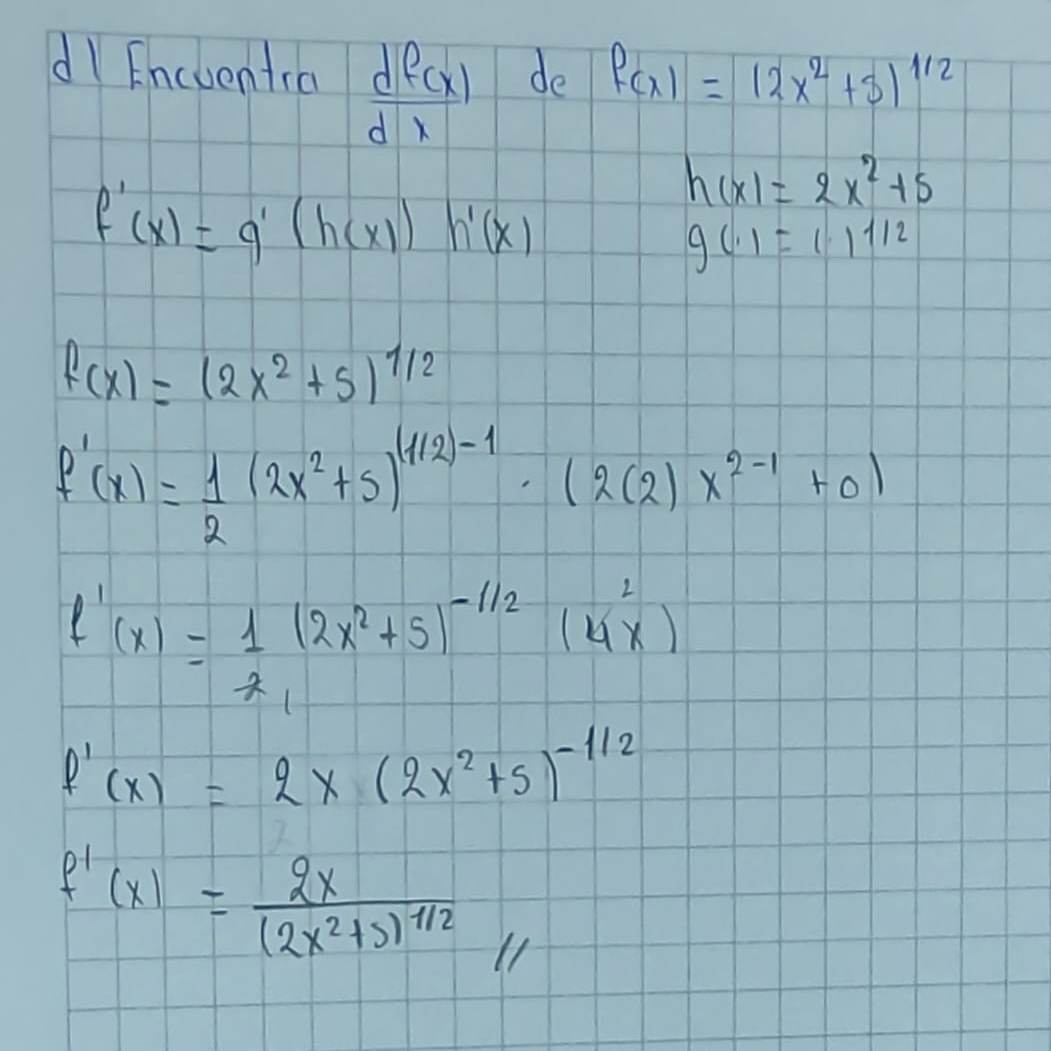
\includegraphics[width=1.14\linewidth]{/Pregunta_7/7_d.png}
	\end{figure}
\end{enumerate}

\section*{Pregunta 8}
Calcula llas siguientes derivadas parciales. No es necesario simplificar.

\begin{enumerate}[label=(\alph*)]
	\item Encuentra $\frac{\partial z}{\partial x}$ y $\frac{\partial z}{\partial y}$ de $z=3^2+2y^3$
	\begin{figure}[H]
		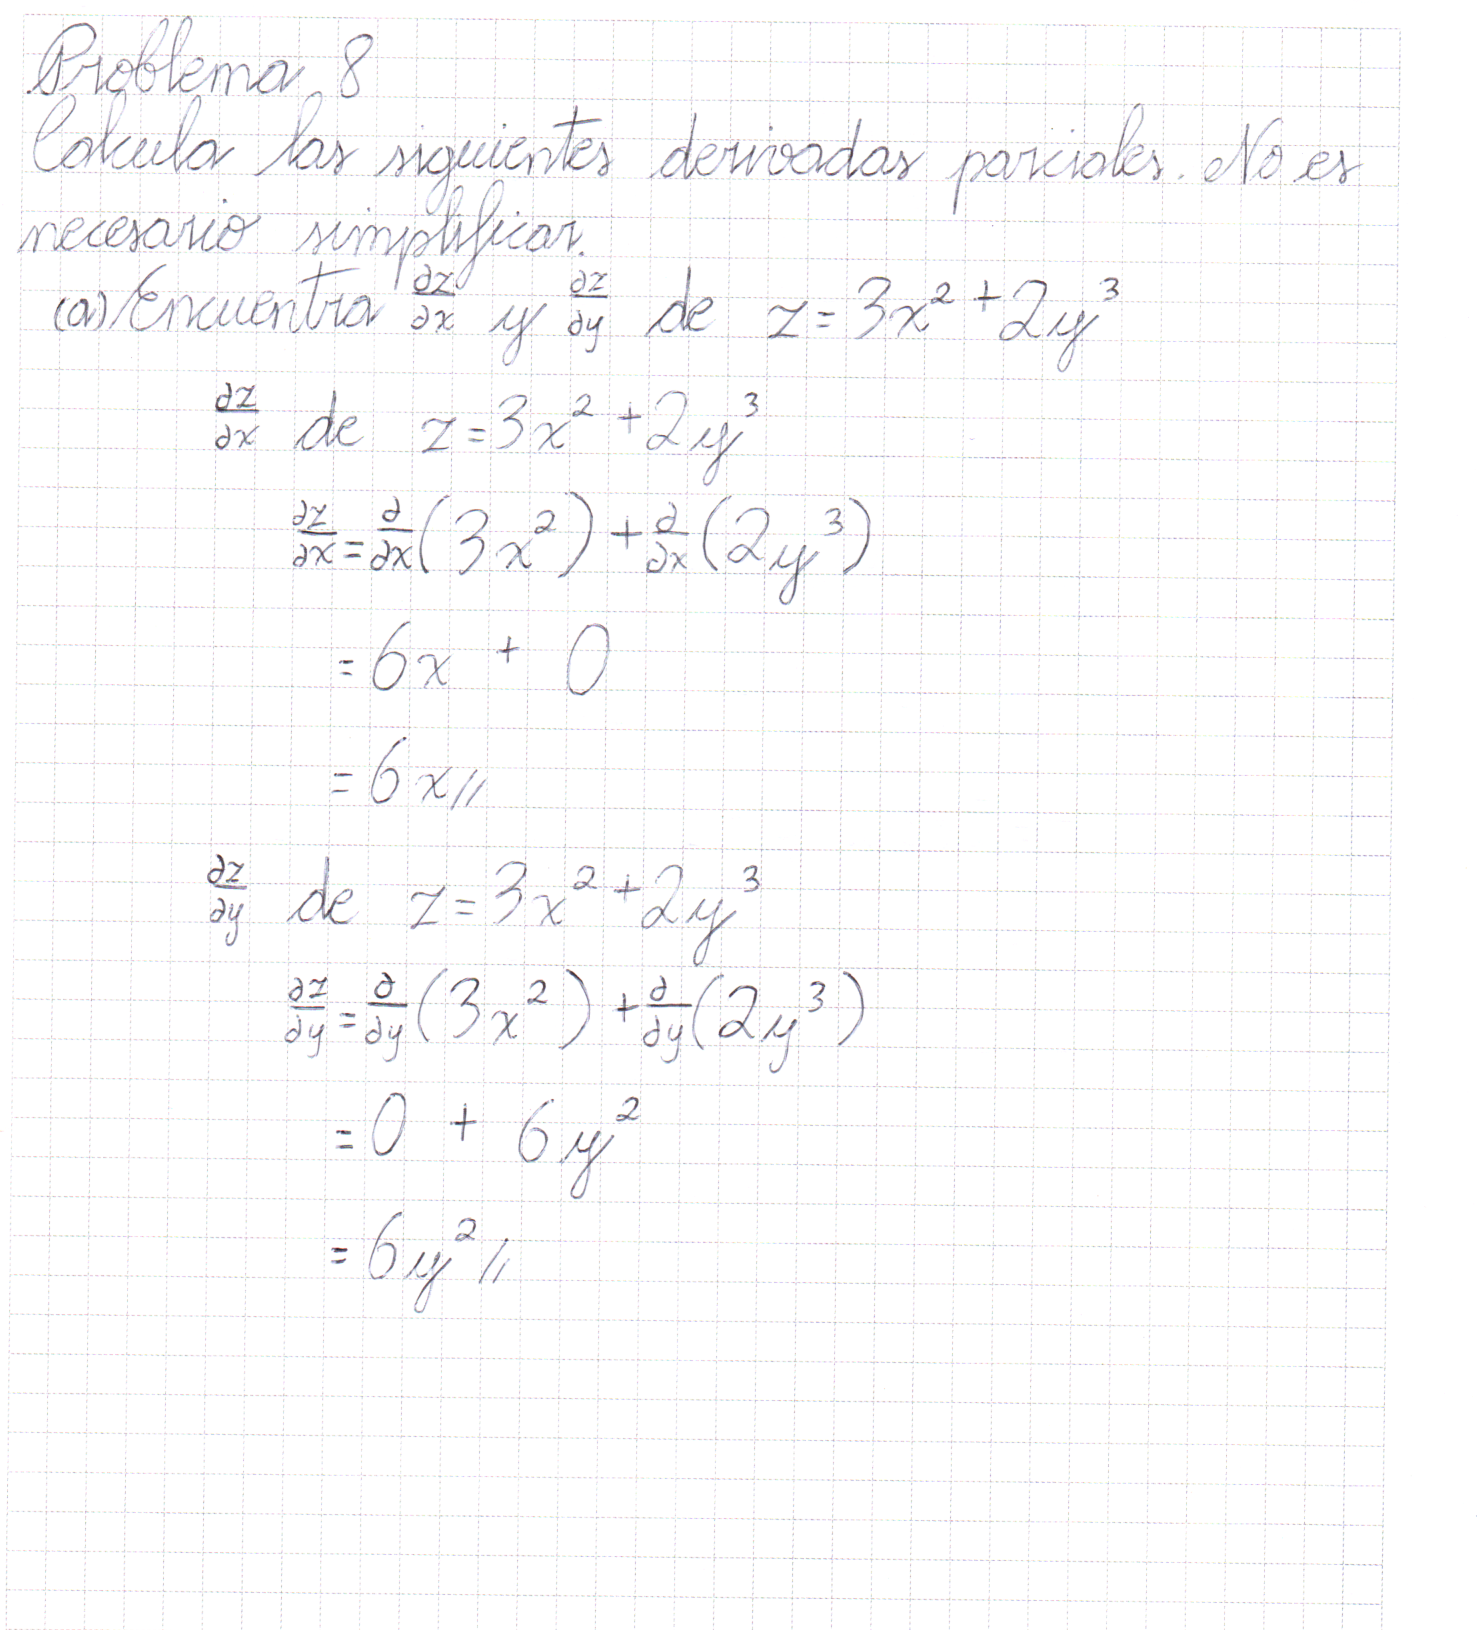
\includegraphics[width=1\linewidth]{/pregunta_8/8_a.png}
	\end{figure}
	\item Encuentra $\frac{\partial z}{\partial x}$ y $\frac{\partial z}{\partial y}$ de $z=(3x-y+1)^\frac{1}{2}$.
	\begin{figure}[H]
		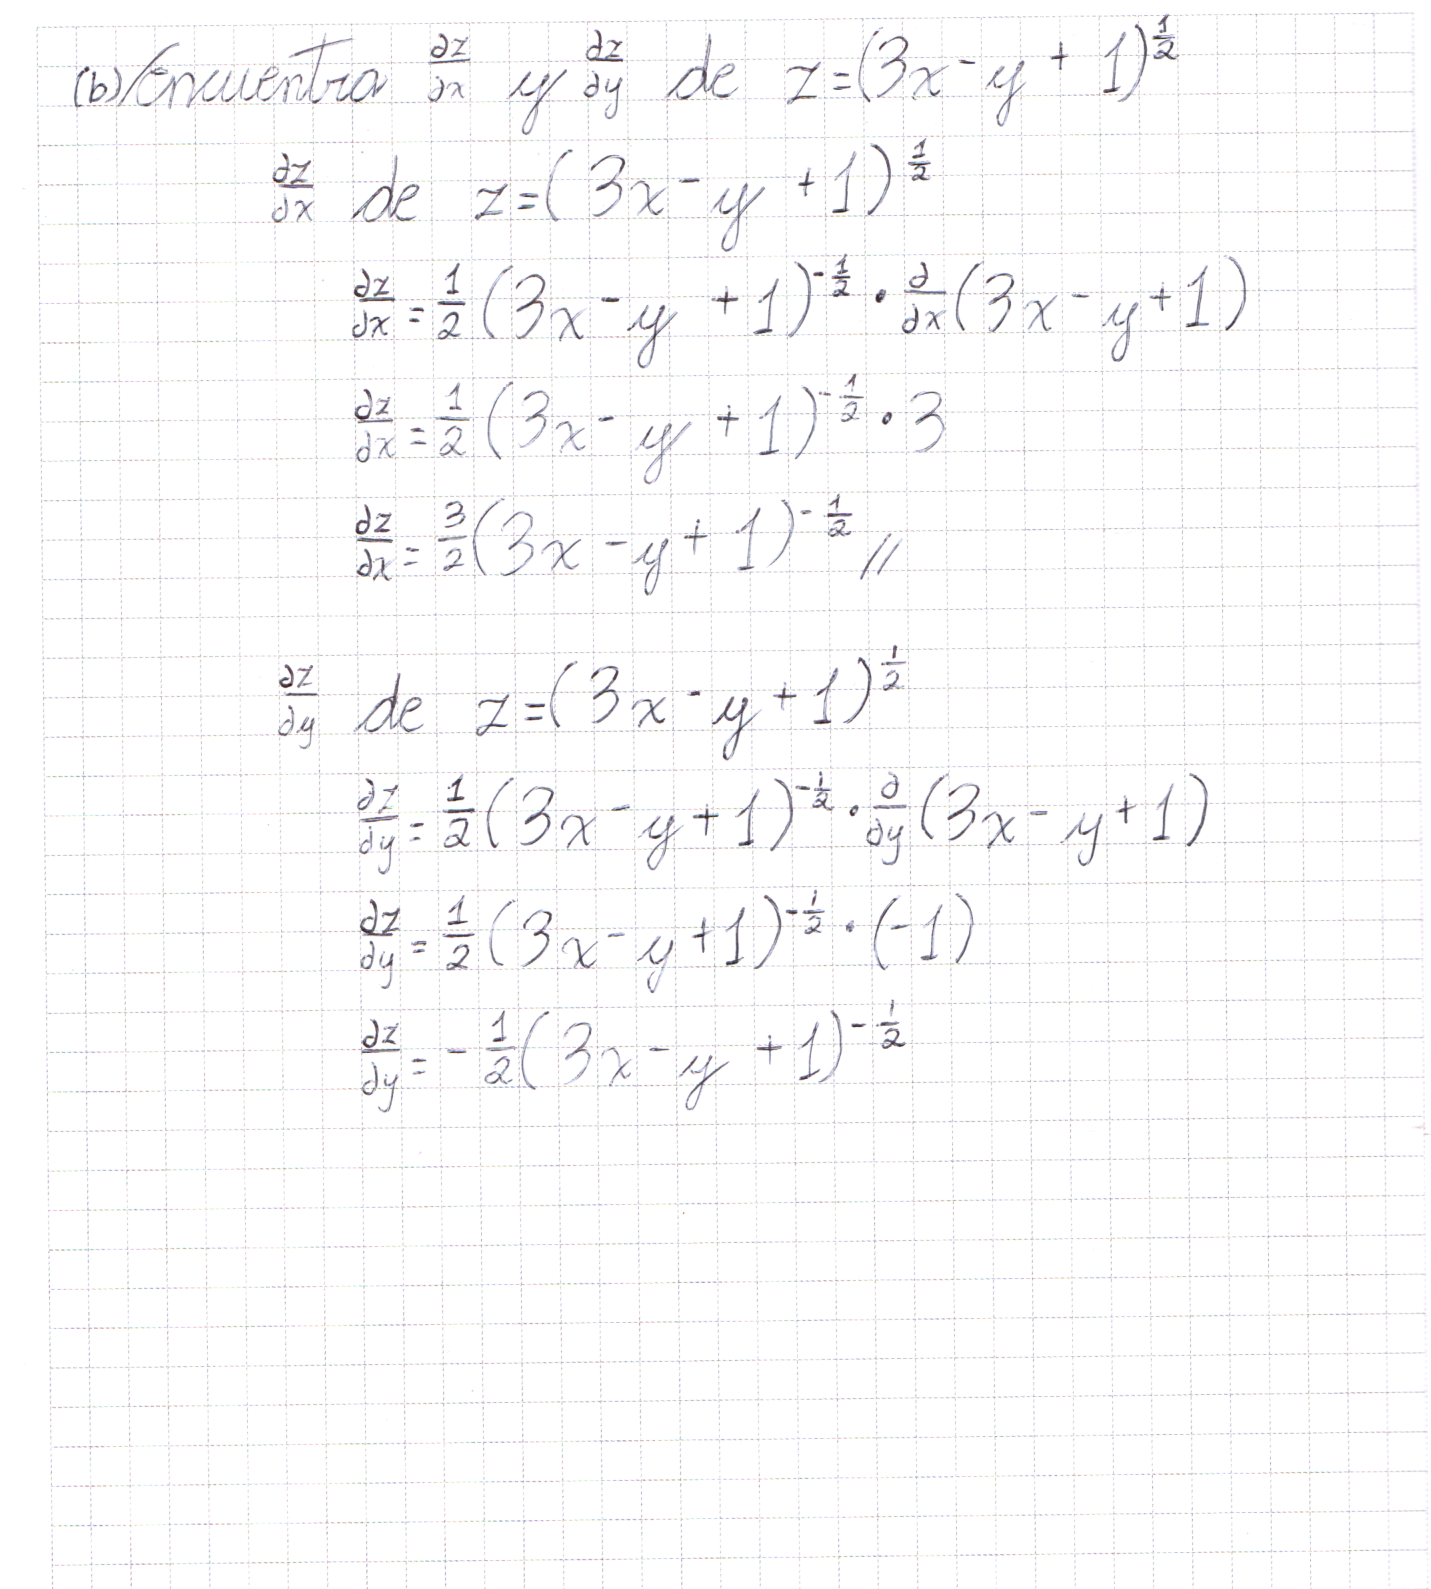
\includegraphics[width=1.1\linewidth]{/pregunta_8/8_b.png}
	\end{figure}
	\item Encuentra $\frac{\partial f}{\partial x}$ y $\frac{\partial f}{\partial y}$ de $f(x,y)=2x^2y+3xy^2$.
	\begin{figure}[H]
		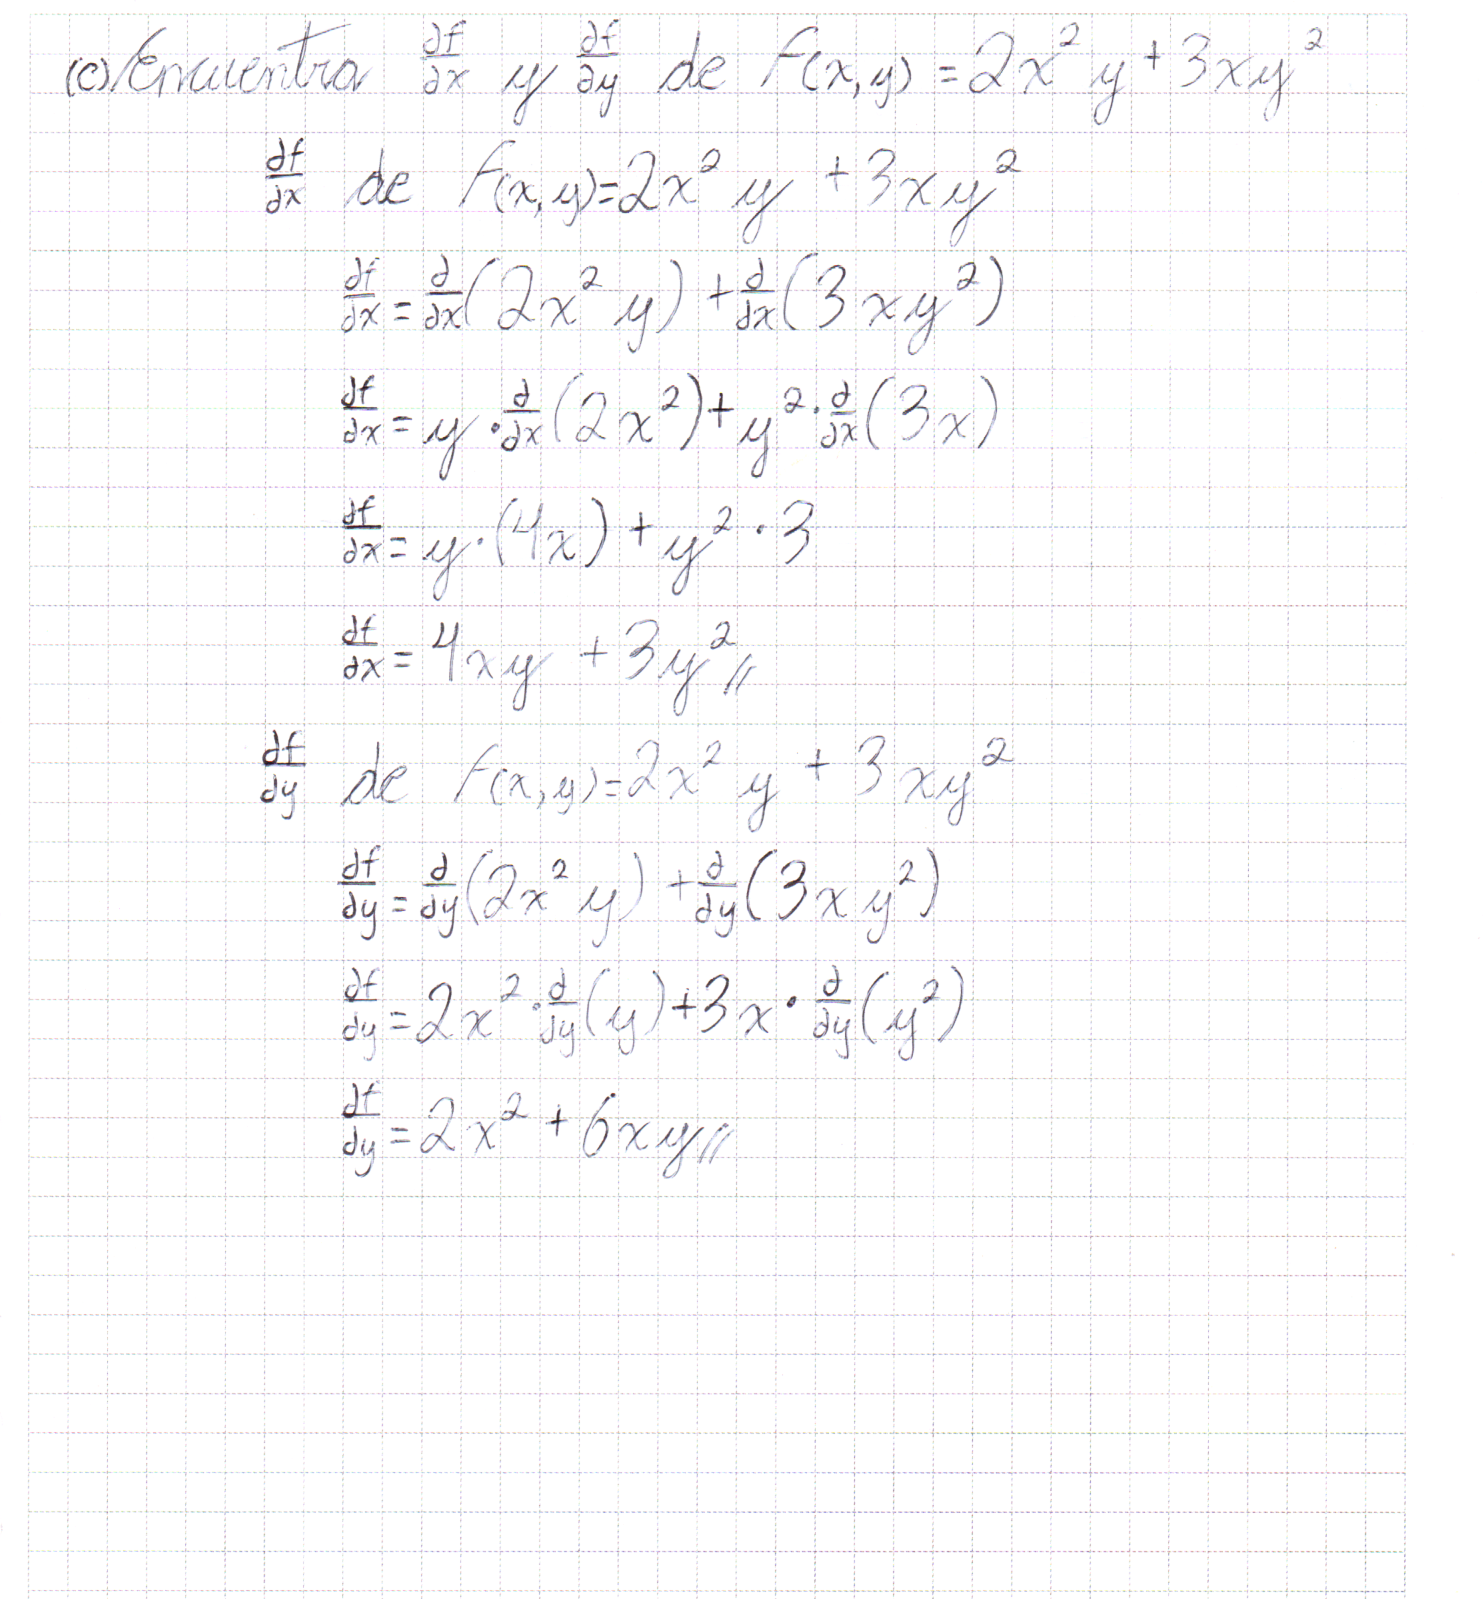
\includegraphics[width=1.1\linewidth]{/pregunta_8/8_c.png}
	\end{figure}
	\item Encuentra $\frac{\partial f}{\partial x}$ y $\frac{\partial f}{\partial y}$ de $f(x,y)=(x^2y^2+2x^3y^2)^2$.
	\begin{figure}[H]
		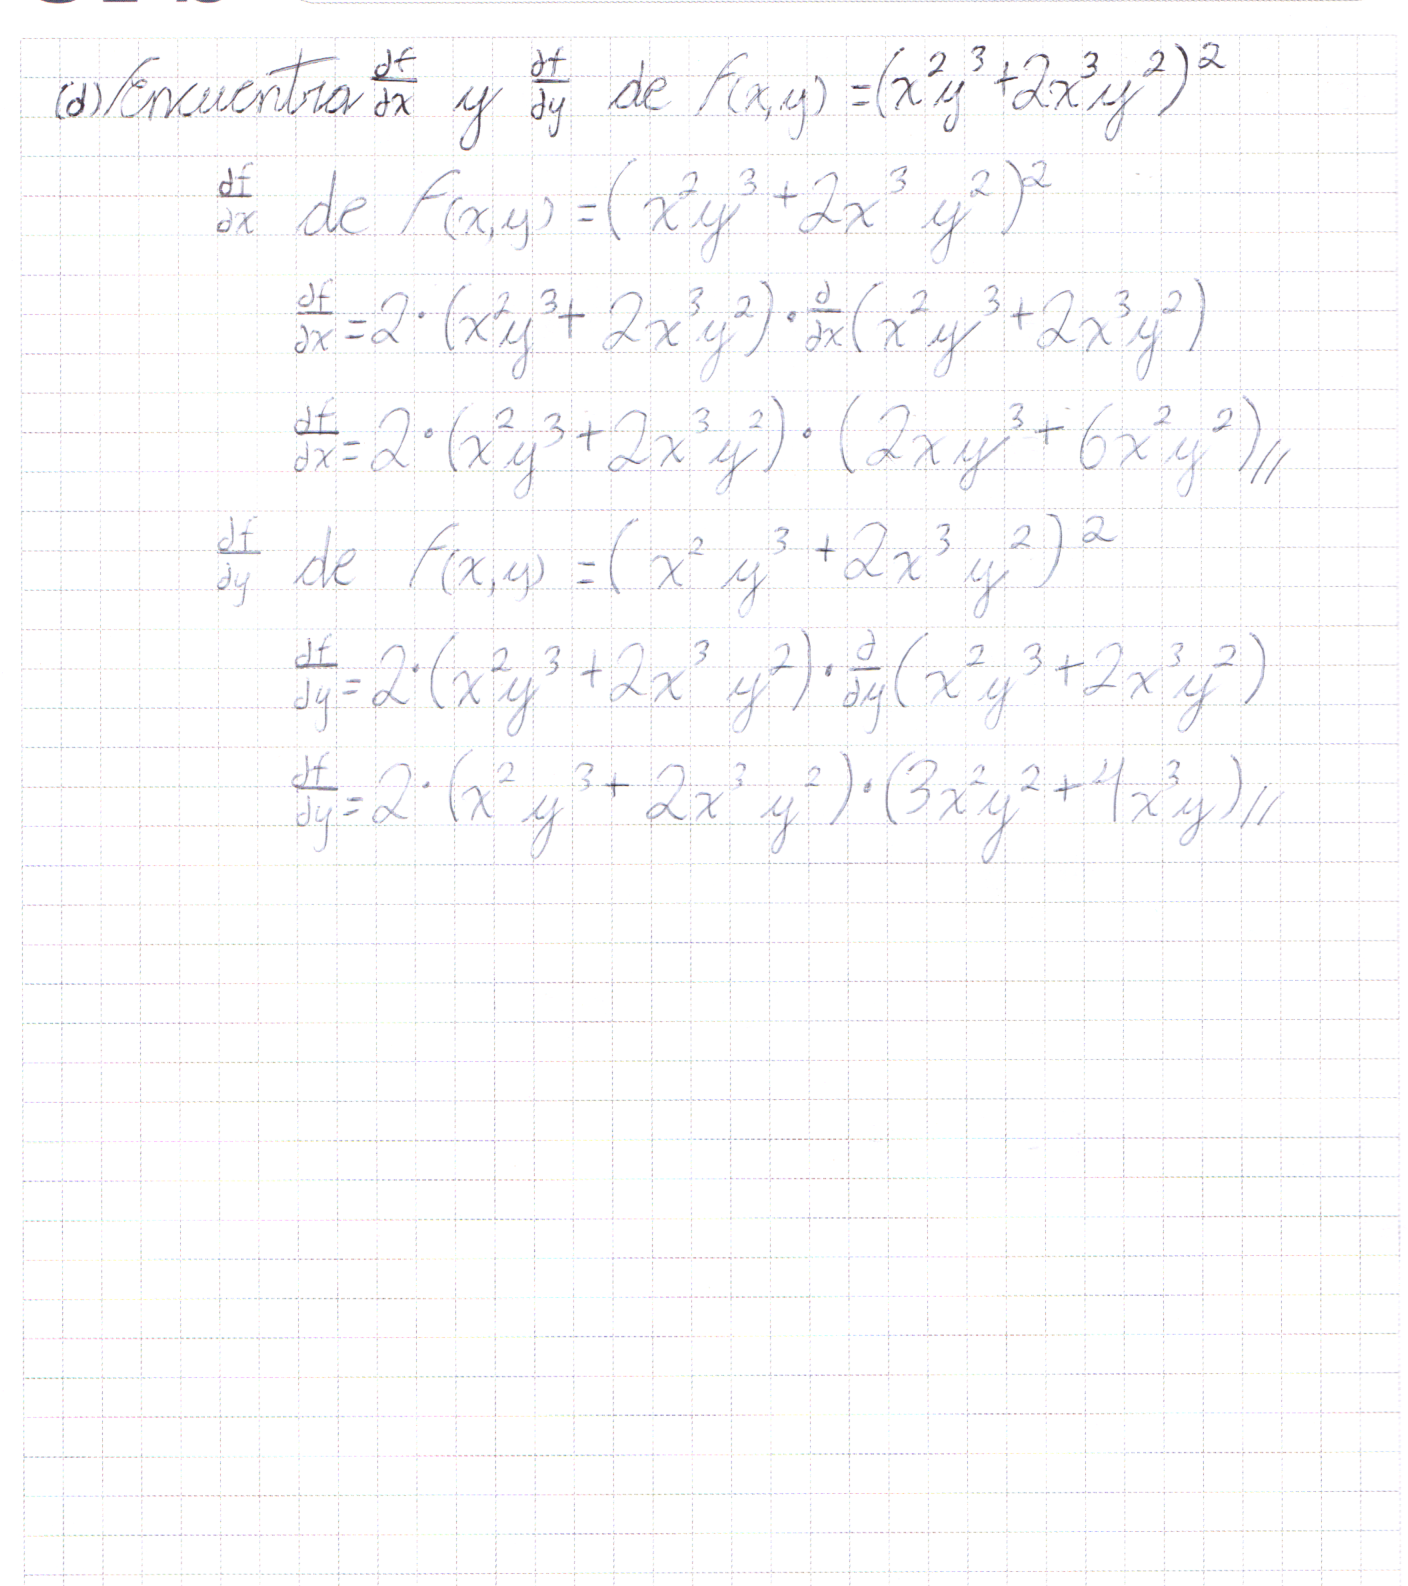
\includegraphics[width=1\linewidth]{/pregunta_8/8_d.png}
	\end{figure}
\end{enumerate}

\section*{Pregunta 9}
Utiliza la derivada de la función para encontrar el valor de $x$ que minimizan la función.

\begin{enumerate}[label=(\alph*)]
	\item Encuentra el valor de $x$ que minimiza la función $f(x)=x^2+4x+5$.
	\begin{figure}[H]
		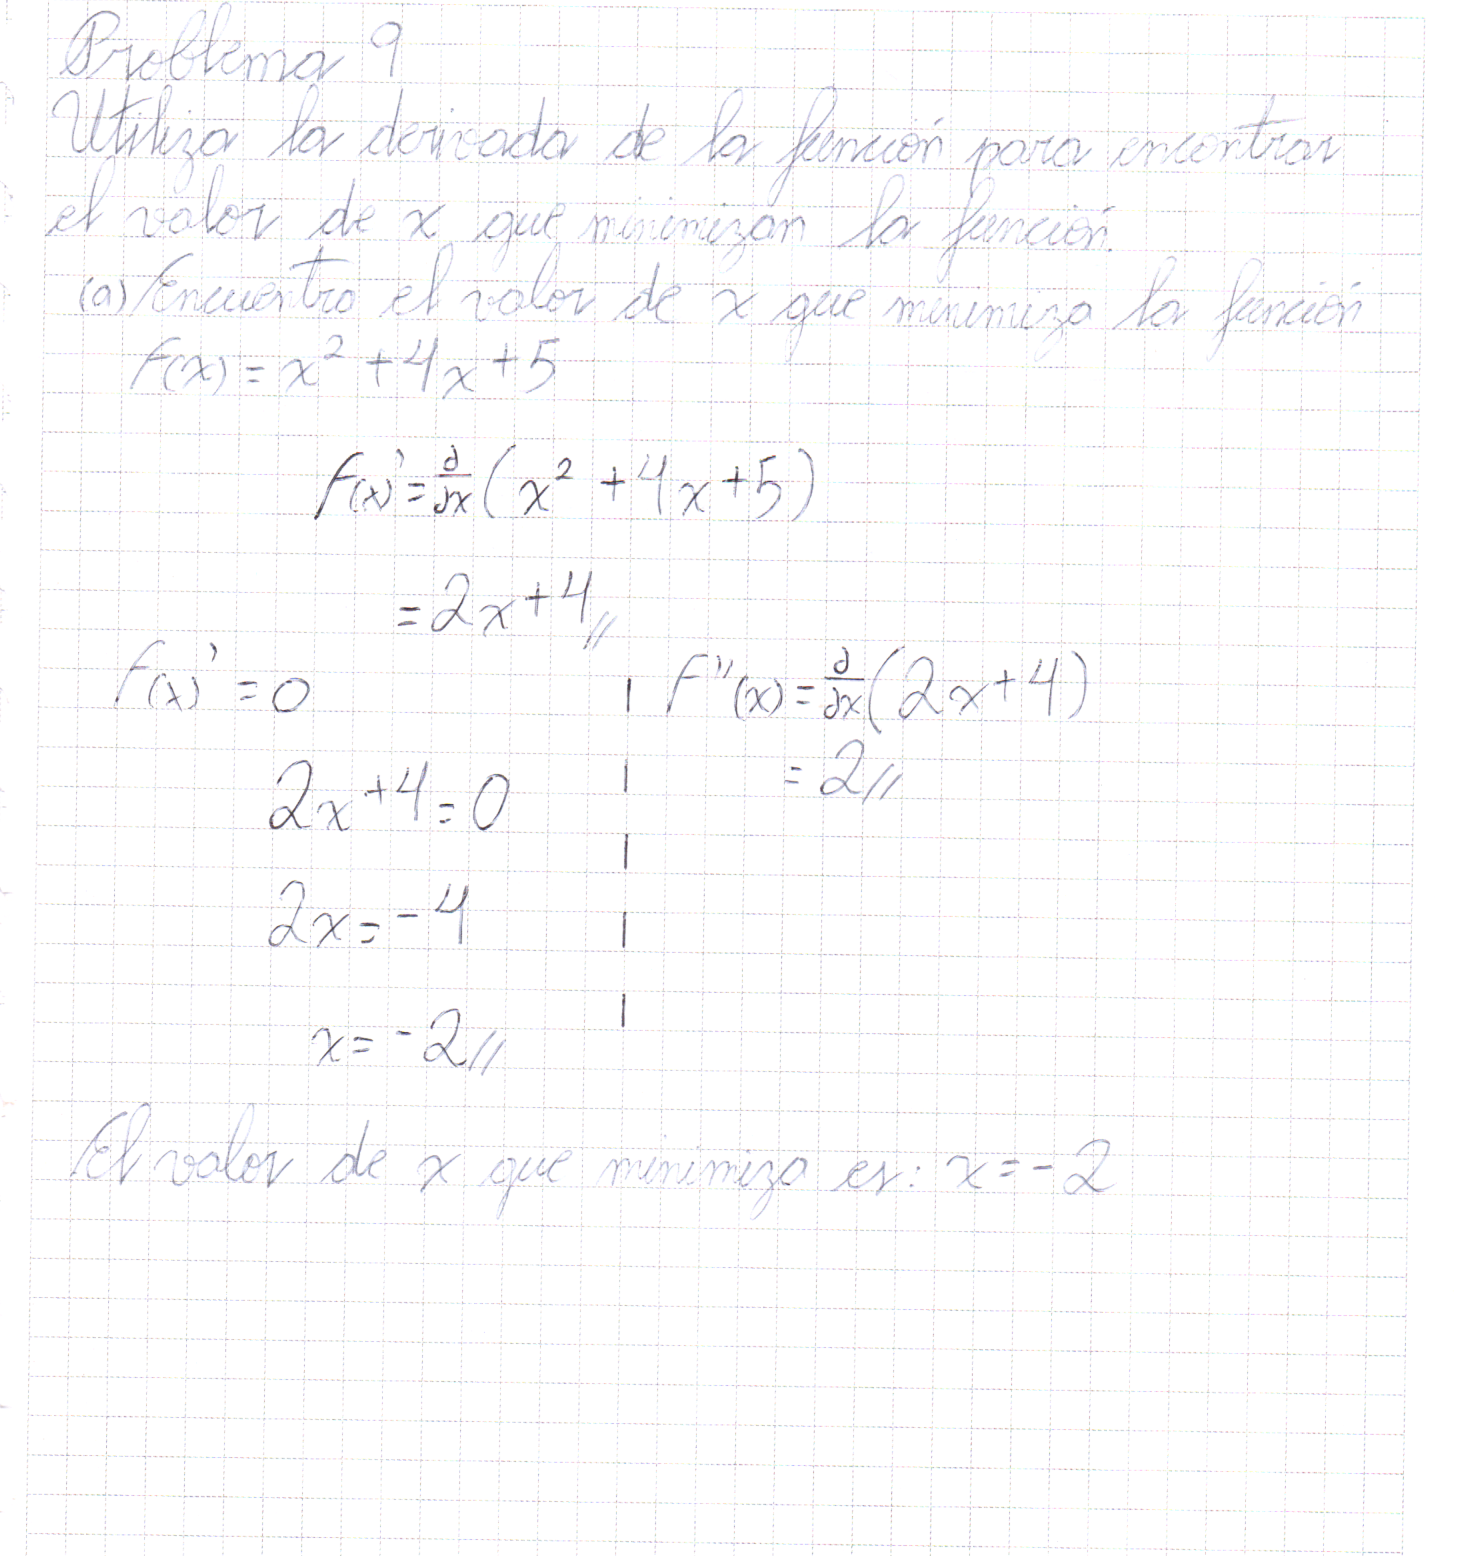
\includegraphics[width=1.06\linewidth]{/pregunta_9/9_a.png}
	\end{figure}
	\item Encuentra el valor de $x$ que minimiza la función $f(x)=(x-3)^2+7$.
	\begin{figure}[H]
		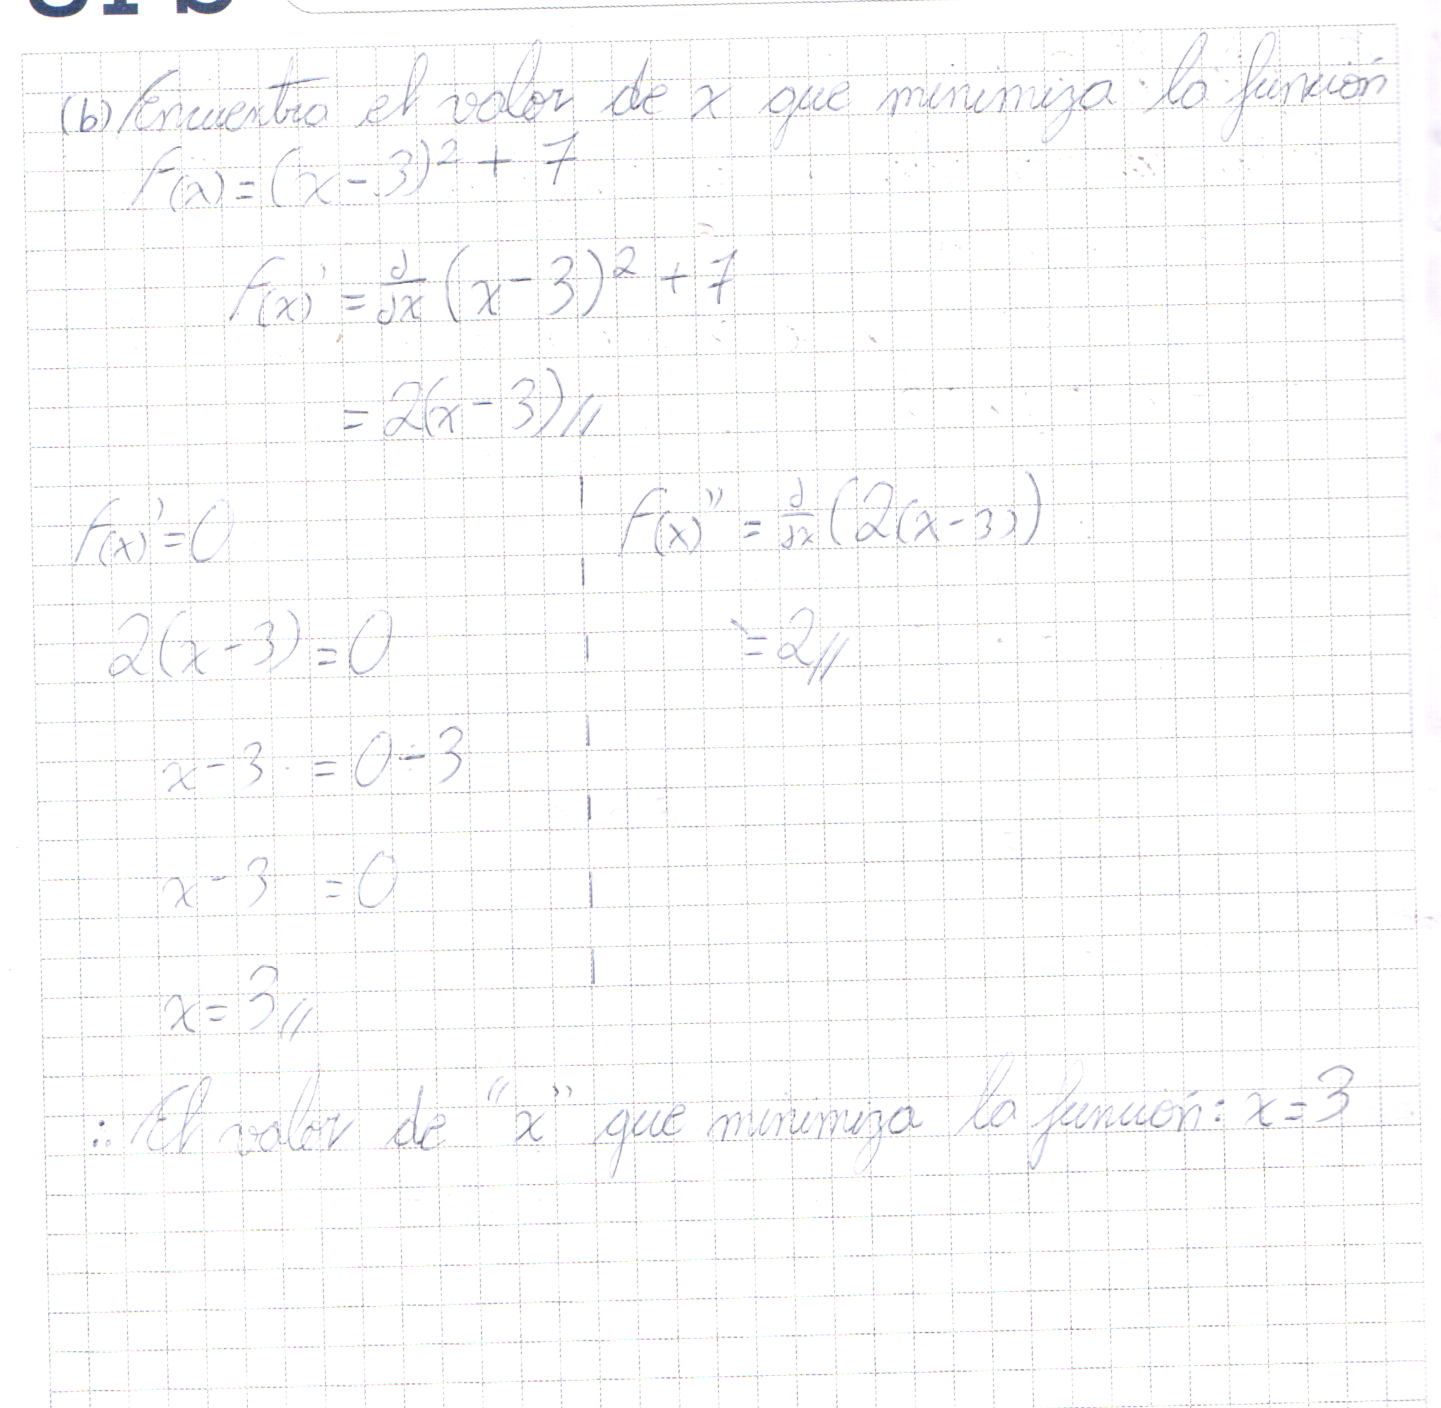
\includegraphics[width=1.15\linewidth]{/pregunta_9/9_b.png}
	\end{figure}
\end{enumerate} 

\section*{Pregunta 10}
Utiliza las derivadas parciales para encontrar los valores $x$ y $y$ que minimizan la función.

\begin{enumerate}[label=(\alph*)]
	\item Encuentra los valores de $x$ y $y$ que minimizan la función $f(x,y)=x^2+y^2$.
	\begin{figure}[H]
		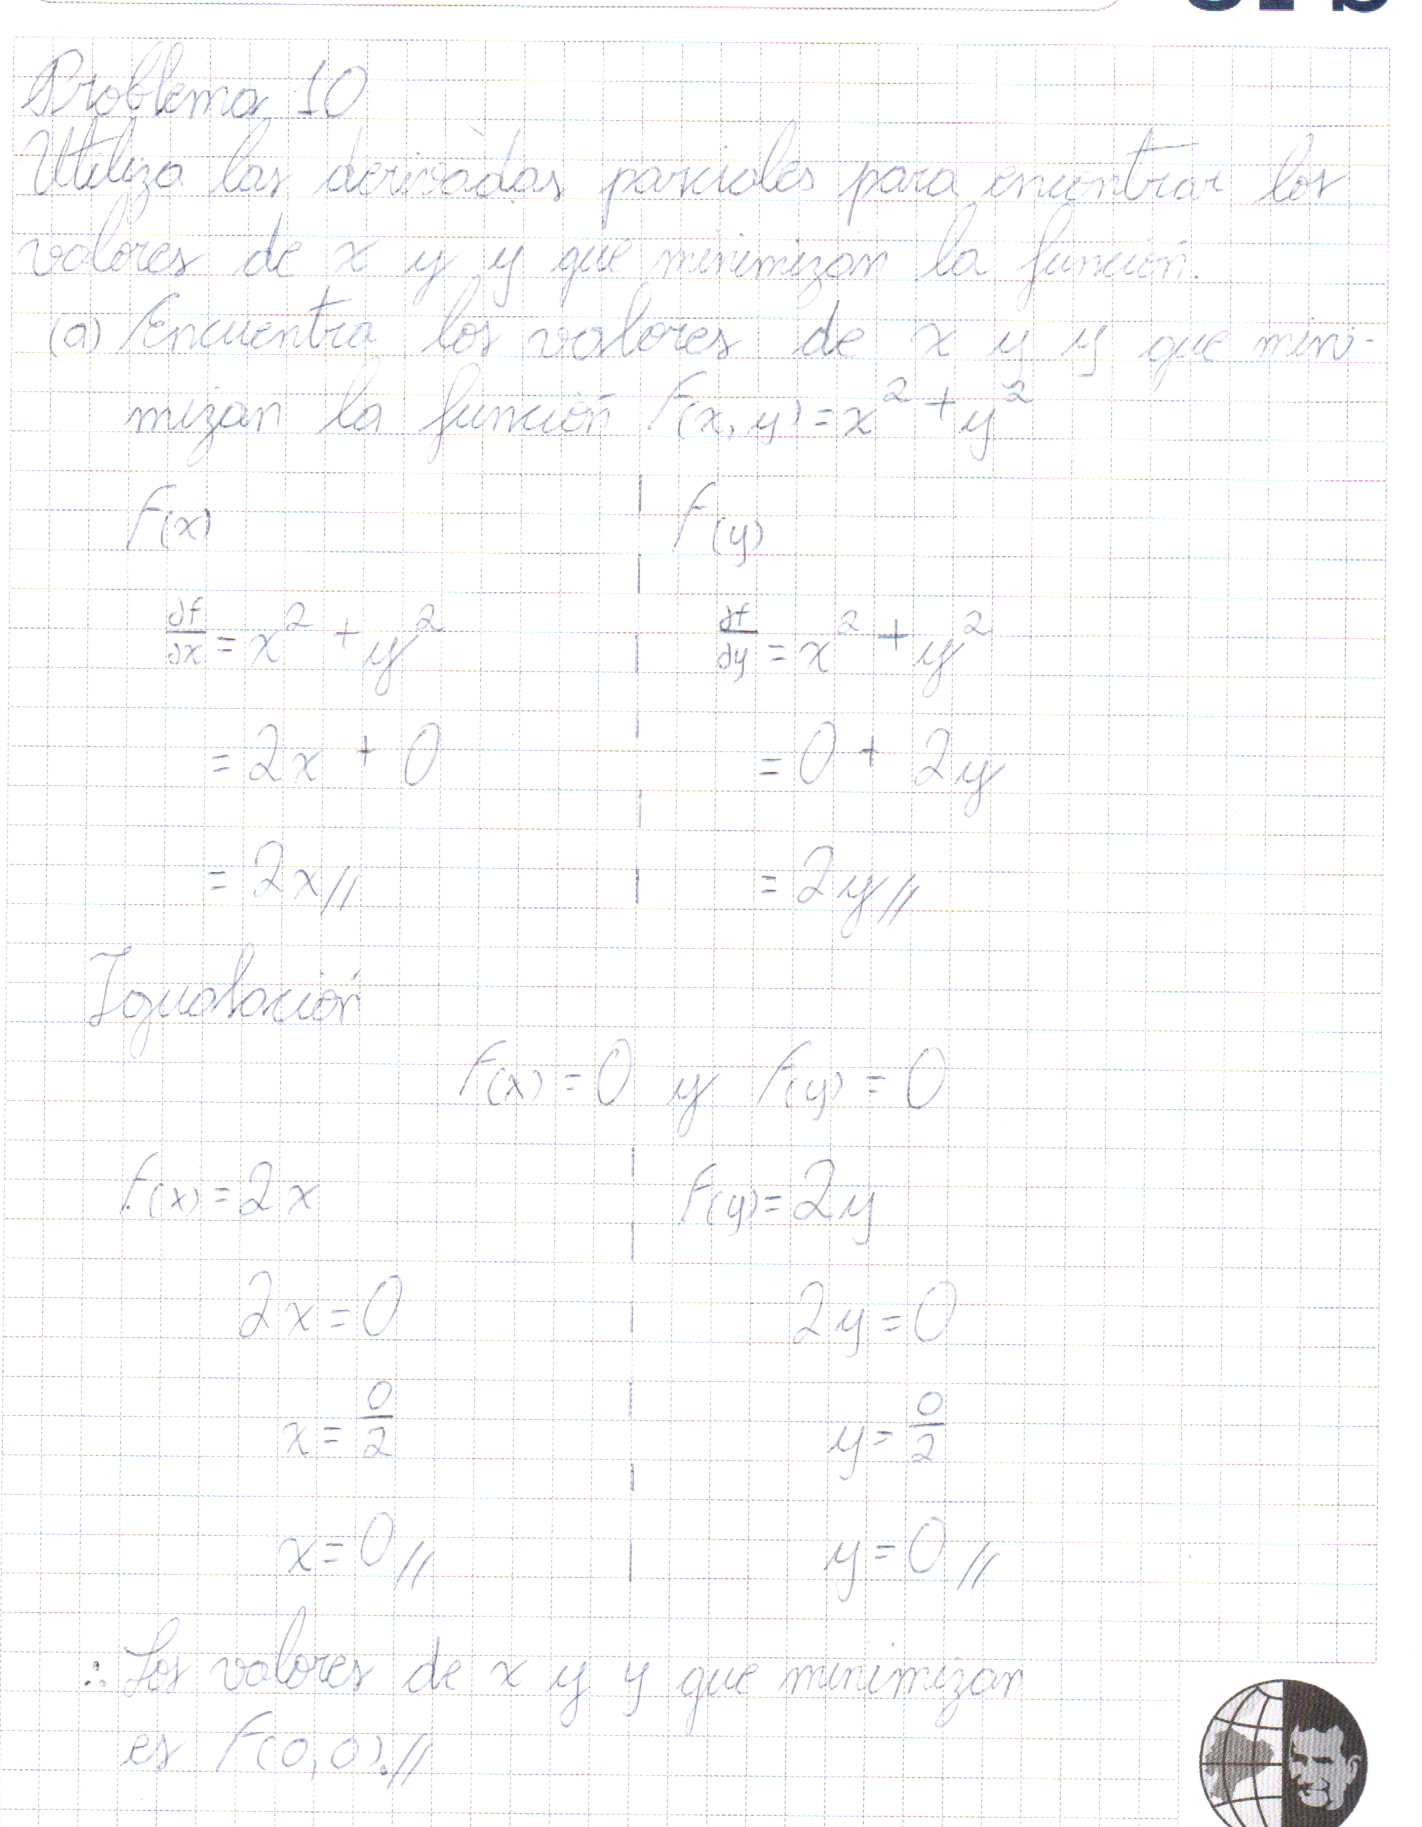
\includegraphics[width=0.86\linewidth]{/pregunta_10/10_a.png}
	\end{figure}
	\item Encuentra los valores de $x$ y $y$ que minimizan la función $f(x,y)=x^2+y^2+4x+6y+14$
	\begin{figure}[H]
		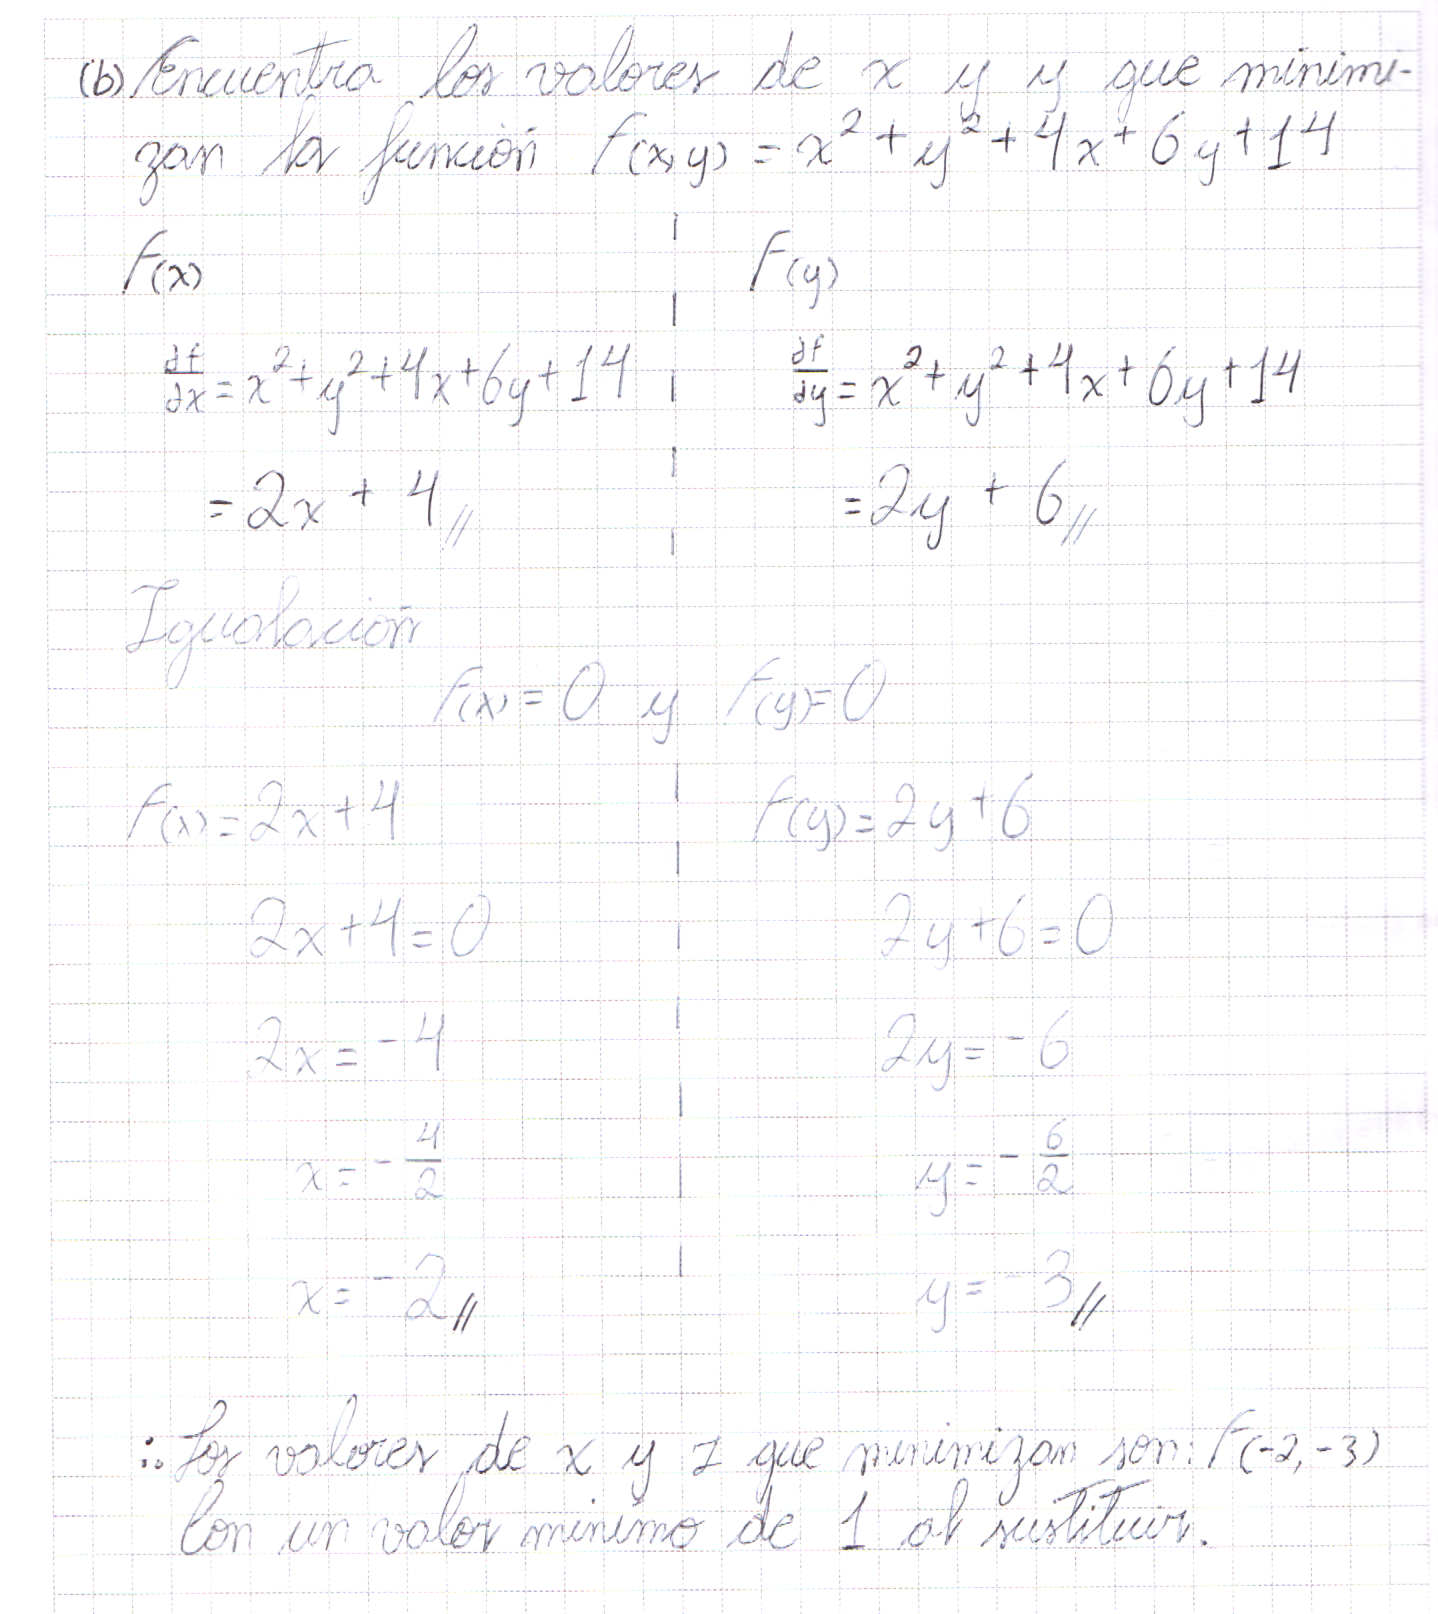
\includegraphics[width=0.98\linewidth]{/pregunta_10/10_b.png}
	\end{figure}
\end{enumerate}
\end{document}
